\documentclass[preprint]{JHEP3} % 10pt is ignored!

\JHEPspecialurl{http://jhep.sissa.it/JOURNAL/JHEP3.tar.gz}
\usepackage{graphicx}
\usepackage{amsmath,amssymb}
\usepackage{cite}
\usepackage{multirow}

%\newcommand{\DF1A}{\Delta F_{1,A}}
%\newcommand{\DF1V}{\Delta F_{1,V}}
%\newcommand{\Dphill}{\Delta \phi_{ll}}
\newcommand{\eps}{\epsilon}
\newcommand{\mrm}{\mathrm}
\newcommand{\rd}{\mathrm{d}}
\newcommand{\Br}{\mathcal{B}}
\newcommand{\GeV}{\mathrm{GeV}}
\newcommand{\TeV}{\mathrm{TeV}}
\newcommand{\pT}{p_{\mathrm{T}}}
\def\DF1A{\Delta F_{1,A}}
\def\DF1V{\Delta F_{1,V}}
\def\Dphill{\Delta \phi_{ll}}
\def\ttbZ{t\bar{t}Z}
\def\ttb{t\bar{t}}
\def\ptZ{p_{t,Z}}
\newcommand{\be}{\begin{eqnarray}}
\newcommand{\ee}{\end{eqnarray}}
%\newcommand{\ttb}{t \bar{t}}

% \title{Constraining top quark-Z boson couplings in $t\bar{t}+Z$ production at the LHC}
\title{Constraining couplings of top quarks to the Z boson in $t\bar{t}+Z$ production at the LHC}

\author{Raoul R\"ontsch \\ Fermilab, Batavia, IL 60510, USA \\
  Email: \email{rontsch@fnal.gov} }
\author{Markus Schulze \\ PH Department, TH Unit, CERN, CH-1211 Geneva 23, Switzerland \\
  Email: \email{markus.schulze@cern.ch} }


\received{\today} 		%%
%\revised{}
\accepted{\today}		%% These are for published papers.


\preprint{CERN Preprint No.xxxxxx\\
FNAL Preprint No.yyyyyy}

\abstract{
We study top quark pair production in association with a Z~boson at the LHC 
%through next-to-leading order QCD
and investigate the prospects of measuring the couplings of top quarks to the Z boson.
To the current date these couplings have never been constrained in direct measurements at hadron colliders.
For the first time, such a determination will be possible at the 13~TeV LHC.
Our calculation improves previous coupling studies through the inclusion of NLO QCD corrections in production and decays of all unstable particles.
We treat top quarks in the narrow width approximation and retain all NLO QCD spin correlations.
To determine the sensitivity of a coupling measurement we perform a statistical log-likelihood ratio test
based on normalization and shape information of the angle between the two leptons from the Z boson.
The obtained limits include the leading theoretical uncertainties from
scale variation and parton distribution functions.
We find that at the 13~TeV LHC with 300~fb$^{-1}$ the vector and axial $t \bar t Z$-couplings can be
constrained to about xx\% and yy\% (1$\sigma$~C.L.), respectively.
Using leading-order input alone these limits deteriorate/worsen/weaken to xx\% and yy\%.
}



\begin{document}
%\maketitle
\section{Introduction}
After run~I and II of the Large Hadron Collider (LHC) at $\sqrt{s}=7$ and 8~TeV we look back at a highly successful research program.
Already this very first phase of exploring a new energy regime has provided many exciting results:
The Higgs boson was discovered, its quantum numbers and couplings are highly constrained,
% and all previously known particles of the Standard Model (SM) were re-discovered within a very short period of time.
and many Standard Model measurements are competitive with previous determinations if not even exceeding them.
Also many minimal extensions of the SM are highly disfavored pushing the scale of new physics to larger values.
This constitues a remarkably fast progress and demonstrates the potential of the LHC in the years to come.

One particularly interesting class of SM processes for which we anticipate more progress in the near future is top quark pair production in association with gauge bosons or a Higgs boson.
% Processes of top quark pairs in association with gauge bosons or a Higgs boson will greatly profit from higher energy and luminosity.
Due to the relatively high production threshold these processes have never been observed with large event numbers at the Tevatron
nor in the current LHC data sample.
In contrast, the high energy and large luminosity of the upcoming LHC run will produce sufficiently many events to allow detailed studies of these processes.
This will open up a new way to directly access electroweak top quark couplings, many of which are only indirectly constrained or not constrained at all.
A few prominent examples are the determination of $Q_t$ in $\ttb+\gamma$ production, measurements of electric and magnetic dipole moments in single top$+\gamma$ production, 
as well as $y_t$ in the $\ttb+H$ process.

% Top quark phenomenology is one prefered corner to look for sign of new physics.
% New dynamics related to el.weak symm. breaking might show up in the top quark sector first.
% LHC experiments have already explored most prominant observables such as top pair inv. mass spectrum, spin correlations and W helicity fractions in top quark pair production. Signatures of top pairs in association with large missing energy are of high interest for
% top partner searches.
% Also single top quark production has been used to look for signs of New Physics [see W' searches].


% This affords the high energy physics community the opportunity to examine the possible future physics reach of the LHC.
% The large top quark production rate at the LHC has allowed detailed study of several of it properties. A combined ATLAS and CMS analysis \cite{ATLAS-CONF-2013-102} has measured the top mass with an accuracy comparable to that obtained at the Tevatron \cite{}. The top electric charge \cite{Aad:2013uza}, $\ttb$ charge asymmetry \cite{CMS-PAS-TOP-12-033}, and $\ttb$ mass difference \cite{Aad:2013eva} have also been measured recently. {\bf top quarks w dijet?}.

% The large top mass places it in a special position within the electroweak symmetry breaking framework. For this reaon, a direct determination of the coupling of the top quarks to the massive gauge bosons would be extremely interesting.  A significant deviation from the Standard Model (SM) value could be indicative of new physics {\bf some silly susy example here? I don't think its a good idea...}; on the other hand, confirmation of the SM value would place further constraints on any new physics scenario. Both CMS \cite{Chatrchyan:2013qca} and the ATLAS \cite{ATLAS-CONF-2012-126} have observed top-pair events produced in association with a vector boson, albeit with very low statistics. The question then arises: how well can the upcoming run at higher energy and larger luminosity constrain the top-vector boson coupling?

In this paper, we focus on the determination of the top quark $Z$-boson coupling through $\ttbZ$ production at the LHC. +...+
Certain extentions of the SM which adress dynamic electroweak symmetry breaking induce large shifts of order 5-10\% \cite{?}.
% See   http://arxiv.org/abs/hep-ph/0512053v1  for this statement:
% "For example, it is well known that the vector and axial tbtZ form factors receive large corrections (of order 5-10%)
%   in certain models of dynamical electroweak symmetry breaking [1]."  
%  But the reference [1] is useless and does not contain any number!!!
% 
% See also http://prd.aps.org/pdf/PRD/v88/i9/e094007 for more useful references:
% "The top-quark couplings with the gauge bosons can be
% modified significantly in models with new top (or third
% generation) partners. This is the case of some extensions of
% the minimal supersymmetric standard model [3,4], in little Higgs models [5], top-color models [6], top seesaw [7], top compositeness [8], and others. Testing them is therefore of
% paramount importance to find out whether there are other sources of electroweak symmetry breaking that are differ-ent from the standard Higgs mechanism.

It is therefore an interesting question to what extent LHC experiments are sensitive to deviations due to physics beyond the SM.
% or to place exclusion limits. 
Clearly, this is not only a question of experimental sensitivity but it also depends crucialy on our theoretical understanding of the production and decay dynamics of the $pp\to\ttbZ$ process.

The ability of LHC experiments to constrain the top-$Z$ coupling was first considered in a series of leading-order studies by Baur,~Juste,~Orr and Rainwater \cite{Baur:2004uw,Baur:2005wi,one more Baur paper}. 
The authors identified suitable observables which are sensitive to vector and axial couplings as well as to the weak electric and magnetic dipole moments.
The tri-lepton signature with semi-hadronically decaying top quarks and a leptonically decaying $Z$ boson provides the best compromise between
clean signature and large enough cross section. 
But even decay modes with a $Z$ boson decaying into neutrinos seem to yield promissing sensitivity \cite{Baur:2005wi}.
The authors of Ref.~\cite{Berger:2009hi} perform a similar analysis, also studying the correlation between single top~$+Z$ and $\ttbZ$ production to strengthen the limits.

In the context of this work it is important to emphasize that Ref.~\cite{Baur:2004uw} identified the large leading order scale uncertainty in the theoretical predictions 
as the main obstacle to tighter constraints on the top-$Z$ coupling.
It is the aim of this paper to reduce these uncertainties through a NLO QCD calculation for $\ttbZ$ production and decay into a realistic final state with leptons, jets and missing energy.
% The transverse momentum of the $Z$ boson $\ptZ$ and the azimuthal angle between the leptons originating from its decay $\Dphill$ were found to be sensitive to this coupling. This observation, together with the desirability of applying realistic experimental cuts, means that our analysis must take into account the decays of the top quarks and the $Z$ bosons, including all spin correlations. Furthermore, the authors of ref. \cite{Baur:2004uw,Baur:2005wi} identified the large leading order (LO) scale uncertainty in the theoretical predictions as the main obstacle to tighter constraints on the top-$Z$ coupling. To reduce this uncertainty, we perform our calculation to next-to-leading order (NLO) in QCD, including the NLO corrections to the top quark decay products. {\bf something about the paper of Berger et al}
% The $\ttbZ$ coupling is already measured by indirect means, through the decay of {\bf ??? and ref}, which disfavors non-SM values bigger than xx\%. It is worthwhile attempting to corroborate this measurement using a direct determination in $\ttbZ$ production.
The production of $\ttbZ$, with stable top quarks and a $Z$ boson, was previously calculated at NLO QCD accuracy by Lazopoulos, McElmurry, Melnikov, and Petriello \cite{Lazopoulos:2008de}, and  by Kardos, Papadopoulos, and Trocsanyi \cite{Kardos:2011na}.
% Disagreement at the level of 3\% of the cross-section, and a small shape difference in $\ptZ$, was found between these two calculations. 
The latter calculation was also interfaced to a parton shower \cite{Garzelli:2011is}, accounting for the decays of the top quarks and $Z$ boson through the spin uncorrelated parton shower approximation.
Further hadronization effects were studied in Ref.~\cite{Garzelli:2012bn}.
Since our coupling analysis relies on studying leptonic opening angles we believe that spin correlations are crucial for a correct interpretation of the results.
We therefore account for NLO QCD spin correlations in the decay of top quarks and hadronically decaying W bosons.
This particularly includes the full 1-loop corrections as well as additional soft, collinear and wide angle gluon emission off the top quark decay chain.
Spin correlations of the leptonically decaying Z boson are included as well.
While including all spin correlations, we approximate top quarks and the Z boson as close to on-shell in the narrow-width approximation. +...+

% This neglects the contribution from the NLO corrections to the top decays, which are included in our calculation. 
% Furthermore, the parton showering produces isotropic distributions and cannot be used to compare spin-dependent observables, such as the lepton opening angle. 
% This paper then presents the first calculation of NLO effects in $\ttbZ$ production and decay, and including all spin correlations.

The study of top-Z couplings is not the only scenario in which the process $pp\to\ttbZ$ is interesting. 
The semi-hadronic decay mode of the top pairs together with the leptonic Z decay is background to several tri-lepton and same-sign lepton searches with additional jets and missing energy.
Those signatures can arise from gluino decays of Super Symmetry, universal extra dimensions as well as models with fermionic top quark partners. 
Furthermore, the invisible decay $Z \to \nu \bar{\nu}$ produces a top pair plus a large amount of missing transverse energy, and is therefore an irreducible background to searches for 
scalar of fermionic top quark partners decaying into top quarks plus dark matter candidates.
While we do not address this issue in this paper, it would be interesting to study the effects of the NLO corrections on this background, using typical selection  cuts of the experimental searches.

Finally we note, .... [no background, tZ is background, only 1/10, but still interesting...]
The top-$Z$ coupling may also be directly probed through single top production in association with a $Z$-boson. While the inclusive cross-section of $tZ$ plus its charge conjugate process $\bar{t}Z$ is comparable to the inclusive $\ttbZ$ cross-section \cite{Campbell:2013yla}, it should be possible to separate these processes by cutting on forward jets and demanding a high jet multiplicity. We will therefore consider only the $\ttbZ$ process in this paper, and defer the study of the coupling using $tZ+\bar{t}Z$ (or both this and $\ttbZ$) to a later date.

% Pheno motivation: LHC a top factory, new top measurements; possibility of measuring top couplings; ttbZ $\to \nu \nu$ as background to MET searches for stops. \\
% Previous NLO calc (w/o top or Z decay): LMMP, KTP \\
% Prev. analysis of top-Z couplings: Baur et al, Berger et al \\
% Comparison with indirect constraints on top-Z coupl \\
% Single top+Z \\

\section{Outline of the calculation}
In this section, we brielfy discuss the features of our calculation.
We consider the tri-lepton signature  
$pp \to \ttb + Z \to t(\to \ell \nu b) \, \bar{t} (\to jj \bar{b}) \, Z(\to \ell \ell)$
which profits from a large cross section due to the hadronic decay of one $W$ bosons and the lepton multiplicities from the remaining $W$ and $Z$ boson.
In our results we will sum over all combinations of $e^\pm$ and $\mu^\pm$ in the final state, allowing either $t$ or $\bar t$ to decay leptonically.
Application of the narrow-width approximation for top quarks and the $Z$ boson allows us to separate production and decays stage according to 
\be
 \rd \sigma_{pp\to\ell\ell\ell\nu b \bar{b} jj} = \rd \sigma_{pp\to\ttb+Z} \; \rd\Br_{t\to b \ell\nu} \; \rd\Br_{\bar{t} \to \bar{b} jj} \; \rd\Br_{Z\to \ell\ell}
 \quad+\quad \mathcal{O}(\Gamma_t/m_t, \, \Gamma_Z/M_Z)
, \label{Xsec}
\ee
where $\rd \sigma$ denotes the production cross section and $\rd\Br_{X\to Y}= \rd \Gamma_{X\to Y} \big/ \Gamma^\mrm{tot}_X$ are the partial branching fractions.
The use of the NWA neglects contributions which are parameterically suppressed by $\mathcal{O}(\Gamma / m)$ arising from a largely off-shell top quark or $Z$ boson.
Severe selection cuts on final state particles can violate this approximation when distorting the Breit-Wiegner line shape of the resonance.
In our analysis we aim for a large cross section and only place mild cuts required by experimental detector acceptance. 
Hence, we believe the narrow-width is an excellent approximation for our study\footnote{
If necessary we can improve our results by allowing off-shell top quarks, Z boson and photons at LO.
Non-factoriable corrections at NLO QCD which are suppressed by $\alpha_s \, \Gamma/m$ have to be neglected in our framework.
}.
% These effects can affect large shape changes in distributions that are sensitive to the top mass, such as the mass of the bottom-$W$ system \cite{AlcarazMaestre:2012vp,Papanastasiou:2013dta}. 
% Since we shall only concern ourselves with leptonic distributions and overall cross-sections, such effects do not warrant concern. We also employ the NWA in the leptonic decay of the $Z$ boson. We therefore neglect final state leptons which arise through an intermediate photon. Such effects are negligible if the a mass cut is placed on the lepton pair
We also neglect the contribution from the decay $t \to Wb+Z$ since the available phase space for on-shell top quarks is tiny and $\Br_{t\to W bZ } \approx 3 \times 10^{-6}$ \cite{see Baur}.



\subsection{NLO correction}
At LO, the production of $\ttbZ$ occurs through the $gg$ and $q\bar{q}$ partonic channels. 
At NLO QCD, these channels receive real and virtual corrections, while real emission corrections open up the partonic channels $qg$ and $\bar{q}g$. 
We also include NLO QCD corrections to the top quark decays and the hadronically decaying $W$ boson, consequently their total widths are included at LO and NLO as well.
Eq.~(\ref{Xsec}) expanded up to NLO QCD reads,
\be
 \rd \sigma_{pp\to\ell\ell\ell\nu b \bar{b} jj}^\mrm{NLO} &=& 
 \rd \sigma_{pp\to\ttbZ}^\mrm{LO} \; \rd\Br_{t\to b \ell\nu}^\mrm{LO} \; \rd\Br_{\bar{t} \to \bar{b} jj}^\mrm{LO} \; \rd\Br_{Z\to \ell\ell}
 \; \left( 1 + \chi \right)
\nonumber \\
 &+&   \rd \sigma_{pp\to\ttbZ+X}^{\delta \mrm{NLO}}  \, \rd\Br_{t\to b \ell\nu}^\mrm{LO} \; \rd\Br_{\bar{t} \to \bar{b} jj}^\mrm{LO} \; \rd\Br_{Z\to \ell\ell}
\nonumber \\
 &+&  \rd \sigma_{pp\to\ttbZ}^\mrm{LO} \; \left(  \rd\Br_{t\to b \ell\nu+X}^{\delta\mrm{NLO}} \; \rd\Br_{\bar{t} \to \bar{b} jj}^\mrm{LO} + \rd\Br_{t\to b \ell\nu}^\mrm{LO} \; \rd\Br_{\bar{t} \to \bar{b} jj+X}^{\delta\mrm{NLO}} \right) \rd\Br_{Z\to \ell\ell}
. \label{XsecNLO}
\ee
The factor $\chi= -2 \Gamma_t^{\mrm{tot},\delta\mrm{NLO}}/\Gamma_t^{\mrm{tot,LO}} -2 \Gamma_W^{\mrm{tot},\delta\mrm{NLO}}/\Gamma_W^{\mrm{tot,LO}} $ arises from the $\alpha_s$ expansion
of the total widths in the denominator.
The virtual corrections are evaluated using a numerical OPP realization \cite{Ossola:2006} of $D$-dimensional generalized unitarity \cite{Ellis:2007br,Giele:2008ve,Ellis:2008ir} (for a review, see Ref.~\cite{Ellis:2011}).
We extended the framework of \cite{Melnikov:2009dn} to account for color neutral bosons which requires new tree level recursion relations as well as an extention of the OPP procedure as described in e.g. Ref.~\cite{}.
Soft and collinear singularities in the real emission corrections are regularized using the dipole subtractions scheme of Refs.~\cite{Catani:1996vz,Catani:2002hc} supplemented with a cut-off parameter for the
finite dipole phase space~\cite{Nagy:2003tz,Nagy:2003tz,copy from ttbphoton paper}.
The virtual and real corrections to the top quark decay and hadronic W decay are implemented analytically. Soft and collinear singularities in the real emission phase space are regularized using subtractions dipoles given in~\cite{see ttbphoton paper}.
% The NLO amplitudes for the decay of the top quarks well-known, and are given in \cite{Jezabek:1988iv,Czarnecki:1990pe,Czarnecki:1990kv,Li:1990qf,Campbell:2004ch,}. In the NWA, the NLO cross-section for the production and decay is written as \cite{Campbell:2004ch,Melnikov:2009dn}
\\
We perform several checks to ensure the correctness of our calculations. 
The squared amplitudes for the tree level and real emission corrections are checked against MadGraph~\cite{Alwall:2011uj}. 
The cancellation of poles in $D-4$ of dimensional regularization between the virtual corrections and integrated dipoles has been verfied for several phase space points.
We also checked the finite part of the virtual amplitudes against the automated program {\tt GoSam} \cite{Cullen:2011ac} for a few phase space points.  
At the level of the integrated cross section, we vary the cut-off parameter for the finite dipole phase space by at least one order of magnitude and 
verify independence on this parameter for the total cross section and kinematic distributions.
The implementation of production and decay amplitudes is checked by integrating over the full phase space and verifying the factorization into 
inclusive cross-section for stable top quarks and $Z$ boson times by their branching ratios, at NLO QCD.
% 
Finally, we compare our results with previous calculation in the literature for stable top quarks and $Z$ boson.
This calculation was first performed in Ref.~\cite{Lazopoulos:2008de}. 
For completeness, we repeat the parameters used in that calculation. 
The masses of the top quark, $W$ boson and $Z$ are $m_t=170.9$ GeV, $m_W=80.45$ GeV, and $m_Z=91.19$ GeV. 
The electroweak coupling is defined through the Fermi constant $G_F$ and the weak mixing angle $\sin^2\theta_w = 1-m_W^2/m_Z^2 =0.2215$. 
The MSTW2004 parton distribution functions are used \cite{}, giving a strong coupling $\alpha_s(m_Z)=$ at LO and $\alpha_s(m_Z)=$ at NLO. 
At the central factorization and renormalization scale of $\mu_0=m_t+m_Z/2$, the cross-section was found to be 808 fb at LO and 1090 fb at NLO, leading to a $k$-factor of 1.35. 
The calculation was repeated in Ref.~\cite{Kardos:2011na}.  
Using the same set of parameters as Ref.~\cite{Lazopoulos:2008de}, agreement with the LO cross-section was found. 
However, the NLO cross-section was found to be 3\% higher at 1121 fb, giving a slightly larger $k$-factor of 1.39. 



%OPP, C-S dipoles, top decay at NLO, NWA for tops and Z + Refs \\
% Leptonic, inclusive variables so no need for parton showering \\
%Checks: poles, factorization, alpha-param \\
% Comparison with KTP, LMMP - cross-secs, distr \\

\subsection{Top-Z coupling}
Definition of top-Z couplings - vector, axial-vector, left and right handed \\
Focus of D=4 operators -- D=6 for later (unclear how to implement unitarity for such operators) \\
Definition of DF1V and DF1A

\section{Results}
\subsection{NLO Results}
%TODO:
%Four distr incl scale bounds (incl at least one of a decay product) at LO, NLO\\
%Comparison with NLO + LO decay \\
%Comparison with 0+1 jet from MadGraph using CKKW merging \\
%Acceptance function = $\sigma_{\mathrm{incl}} / \sigma_{\mathrm{cuts}}$ at LO, NLO\\
%Point out large k-factor with cuts than with fully inclusive \\

In this section we describe the details of our numerical analysis and the results.
We consider the process 
$pp \to \ttb + Z \to t(\to \ell \nu b) \, \bar{t} (\to jj \bar{b}) \, Z(\to \ell \ell)$
and sum over all combinations of leptons $e^\pm, \mu^\pm$.
We choose the following fixed input parameter
\be
 m_t = 173~\GeV,& \quad   m_b = 0~\GeV,&
\nonumber\\
 M_Z =91.1876~\GeV,& \quad  M_W =80.385~\GeV,&
\nonumber\\
 G_\mathrm{F} = 1.166379 \times 10^{-5} \,& \GeV^{-2},  \quad \Gamma_Z = 2.4952~\GeV.&
\ee
Unless otherwise stated, we use MSTW2008 parton distribution functions \cite{...} with 
$\alpha_s(M_Z)=0.13939$ and $\alpha_s(M_Z)=0.12018$ at LO and NLO, which we
evolve to the renormalization scale $\mu$ using 1-loop and 2-loop running, respectively.
The LO and NLO scale dependence has already been studied in previous works,
we therefore do not repeat these studies and adopt the central scale \cite{Lazopoulos:2008de}  
$\mu_0=\mu_\mathrm{ren}=\mu_\mathrm{fact}=m_t + M_Z/2$ 
for renormalization and factorization scale in our work.
Since we include NLO QCD corrections to the top quark decay and the hadronically decaying $W$ boson, we need to 
include their total widths up to NLO,
\be
 \Gamma_t^\mathrm{LO} &=& 1.4957~\GeV, \quad \Gamma_t^\mathrm{NLO} = 1.3693~\GeV,
\nonumber\\
 \Gamma_W^\mathrm{LO} &=& 2.0455~\GeV, \quad \Gamma_W^\mathrm{NLO} = 2.1145~\GeV.
\ee
We consider proton-proton collisions at the LHC with a center-of-mass energy of $\sqrt{s}=13~\TeV$.
To account for detector acceptances and trigger we require
\be
 \pT^{\ell} \ge 15~\GeV, \quad |y^{\ell}| \le 2.5,
\nonumber\\
 \pT^{j} \ge 20~\GeV, \quad |y^{j}| \le 2.5,
\nonumber\\
 \pT^{\mathrm{miss}} \ge 20~\GeV, \quad R_{\ell j} \ge 0.4.
\ee
\begin{figure}[t]
\centering % \begin{center}/\end{center} takes some additional vertical space
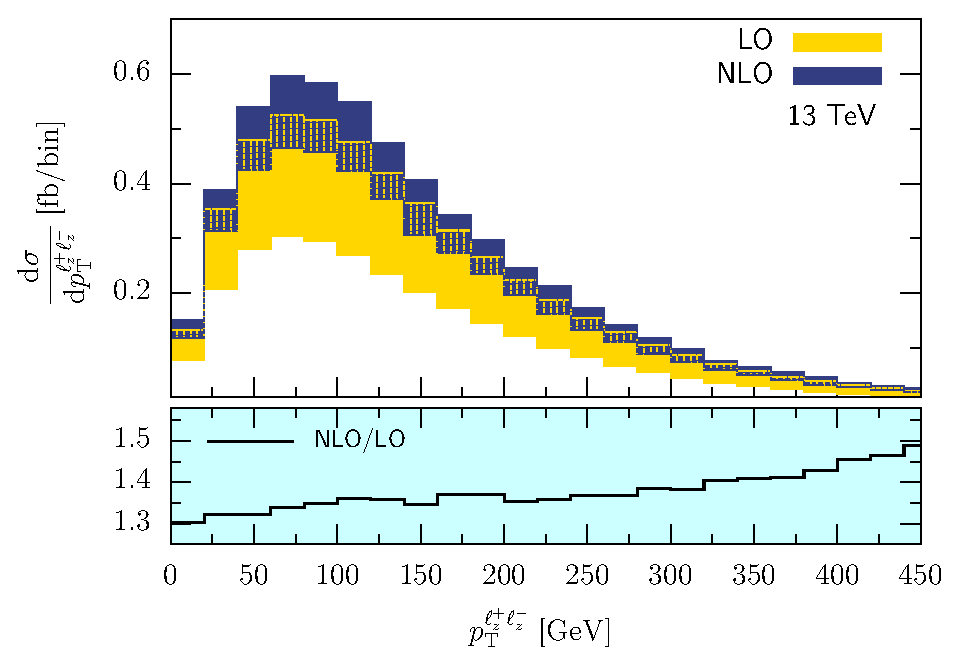
\includegraphics[width=0.45\textwidth]{./LHC_53_Fig12.eps}
\hfill
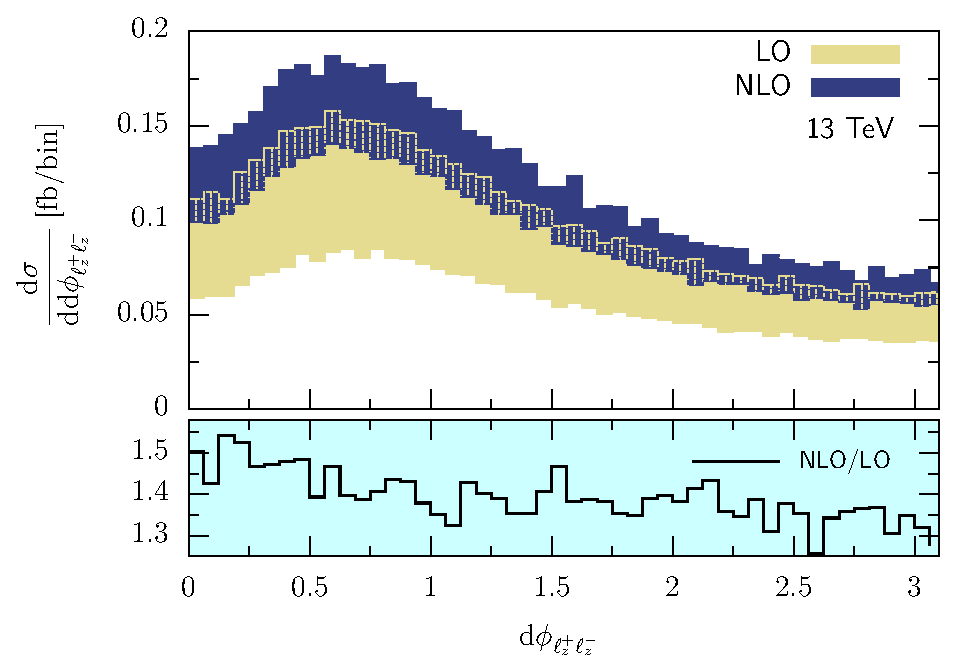
\includegraphics[width=0.45\textwidth]{./LHC_53_Fig17.eps}
\caption{\label{fig:i} Transverse momentum spectrum (a) and azimuthal opening angle (b) of the opposite sign leptons from the $Z$ boson decay
in the process $pp \to \ttb + Z \to t(\to \ell \nu b) \, \bar{t} (\to jj \bar{b}) \, Z(\to \ell \ell)$ at the 13~TeV LHC.
The bands represent the LO (light) and NLO (dark) results for scale variation by a factor of two around the central scale $\mu_0$.
}
\end{figure}
Jet are defined by the anti-$k_\mathrm{T}$ algorithm \cite{Cacciari:2008gp} with $R=0.4$.
With these input parameter and cuts we find the LO and NLO QCD cross sections,
\be
\label{XsecNum}
%  \sigma_{\ttb Z}^\mathrm{LO} &= 3.80^{+1.31}_{-0.94}~\mathrm{fb},
%  \quad\quad\quad
%  \sigma_{\ttb Z}^\mathrm{NLO} &= 5.32^{+0.78}_{-0.74}~\mathrm{fb}
%\\ 
  \sigma_{\ttb Z}^\mathrm{LO} &= 3.80^{+34\%}_{-25\%}~\mathrm{fb},
  \quad\quad\quad
  \sigma_{\ttb Z}^\mathrm{NLO} &= 5.32^{+15\%}_{-14\%}~\mathrm{fb}
%\\ 
%  \sigma_{\ttb Z}^\mathrm{LO} &= 3.98 \pm 28\% ~\mathrm{fb},
%  \quad\quad\quad
%  \sigma_{\ttb Z}^\mathrm{NLO} &= 5.34 \pm 14 \%~\mathrm{fb}
\ee
for the central scale $\mu_0$ which is varied by factors of 2 and $1/2$.
The dependence on the unphysical scale is reduced from approximately $\pm 28\%$ at LO to $\pm 14\%$ at NLO QCD.
Higher order corrections increase the cross section by 40\%, $K= \sigma_{\ttb Z}^\mathrm{NLO} \big/  \sigma_{\ttb Z}^\mathrm{LO}=1.40$.
We also calculate the acceptance function which is given by the ratio of the cross sections in Eq.~\ref{XsecNum} over the 
cross section without any acceptance cuts, 
\be
  A^\mathrm{LO} = \frac{\sigma_{\mathrm{cuts}}^\mathrm{LO}}{\sigma_{\mathrm{total}}^\mathrm{LO}} = 27.2 \% ,
  \quad\quad\quad
  A^\mathrm{NLO} = \frac{\sigma_{\mathrm{cuts}}^\mathrm{NLO}}{\sigma_{\mathrm{total}}^\mathrm{NLO}} = 30.5 \%.
\ee
We supress dependence on the scale variation because it is almost vanishing in the cross section ratios.


Before turning to the $\ttbZ$ coupling analysis, let us discuss some generic kinematic distributions.
Fig.~\ref{fig:i}a shows the transverse momemtum of the two leptons arising from the $Z$ boson.
Similar to the total cross sections we observe a strong reduction in unphysical scale dependence over the entire $\pT$ spectrum.
Scale bands for LO and NLO predictions are comfortably overlapping. 
From this plot we read off a average transverse momemtum of the $Z$ boson of almost 100~GeV with a far extending kinematic tail,
promissing approximately 30 events with $\pT^Z \approx 300~\GeV$ from $300~\mathrm{fb}^{-1}$ at the 13~TeV LHC. 
Fig.~\ref{fig:i}b shows the azimuthal opening angle between the two leptons from the $Z$ boson decay.
This observable has been proven to be a good analyzer of the $\ttbZ$ couplings \cite{Baur:2004uw} and we wil consider it in the following analysis.
The differential $K$-factor in the lower pane of this plot shows shape changes in the range of 10~\% due to higher order corrections.
Shape changes that arise from higher order corrections in the decay matrix elements are shown in the dashed line and amount up to xx\%.


\begin{figure}[t]
\centering % \begin{center}/\end{center} takes some additional vertical space
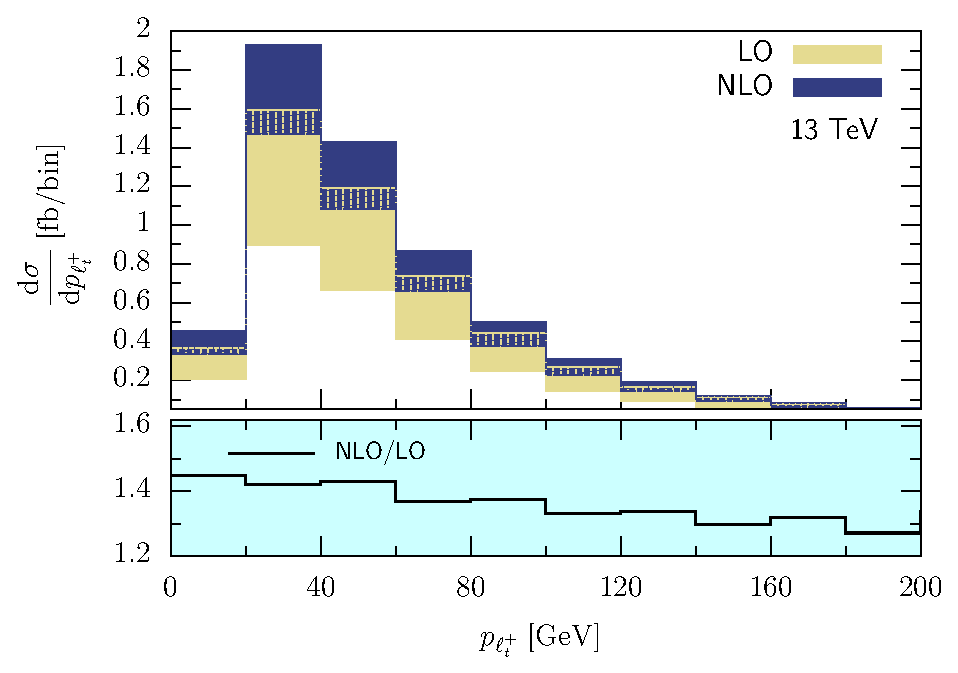
\includegraphics[width=0.45\textwidth]{./LHC_53_Fig01.eps}
\hfill
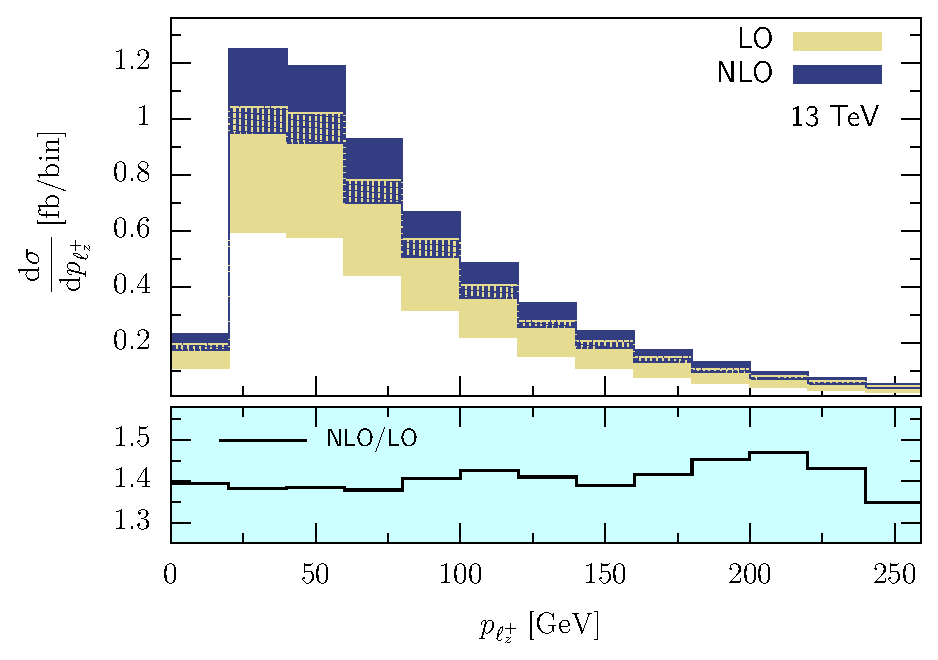
\includegraphics[width=0.45\textwidth]{./LHC_53_Fig03.eps}
\caption{\label{fig:ii} Transverse momentum spectrum of a lepton from the top quark decay~(a) and from the $Z$ boson decay~(b) 
in the process $pp \to \ttb + Z \to t(\to \ell \nu b) \, \bar{t} (\to jj \bar{b}) \, Z(\to \ell \ell)$ at the 13~TeV LHC.
The bands represent the LO (light) and NLO (dark) results for scale variation by a factor of two around the central scale $\mu_0$.}
\end{figure}

In Fig.~\ref{fig:ii}a and Fig.~\ref{fig:ii}b we compare the transverse momentum between the leptons from the top quark and $Z$ boson decay.
We find that leptons from the $Z$ boson have a typically harder spectrum. 
This is already true for LO while significatly different $K$-factors enhance this behavior even further at NLO.


\subsection{Top-Z coupling results}
Constraints from $t\bar{t}Z$ cross-section from CMS \\
Dphill distr with LO and NLO scale bands, and two(three?) non-SM coupl\\
$\sigma_{NP|} / \sigma_{SM}$ a la Berger, 0907.2191 \\
Description of analysis Binned log likelihood, how we handle scale uncertainty (cf. Lykken et al) \\
alpha plots - LO, NLO, rescaled (k-factor and reduced scale uncertainty) LO at 30, 300, 3000 fb-1\\
Dphill distr normalized to $t\bar{t}$ cross-section  - 1 uncertainty from k-factors at 30, 300, 3000\\

\section{Conclusion}
Future work: extension to dim 6 operators, incl single top + Z results, more advanced analysis techniques (e.g. MEM), e+e- collider.
%


\acknowledgments
We acknowledge helpful conversations with Y.~Gao, A.~Gritsan, N.~Tran and P.~Argrawal. 



\appendix
\section{plots}
Temporariy repository for plots.


\begin{figure}[h]
\centering % \begin{center}/\end{center} takes some additional vertical space
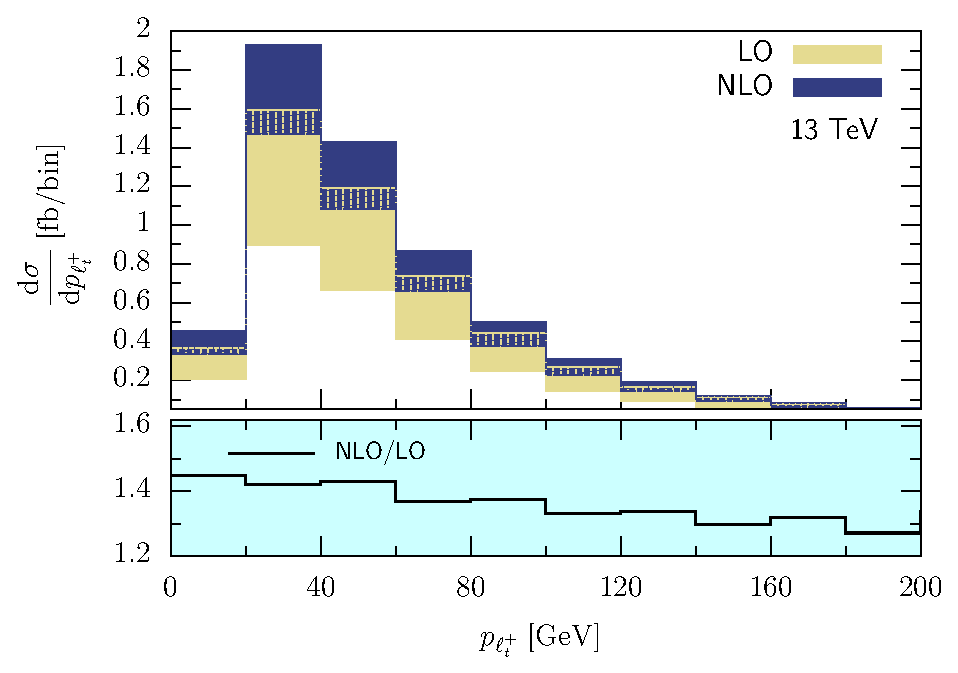
\includegraphics[width=0.45\textwidth]{./LHC_53_Fig01.eps}
\hfill
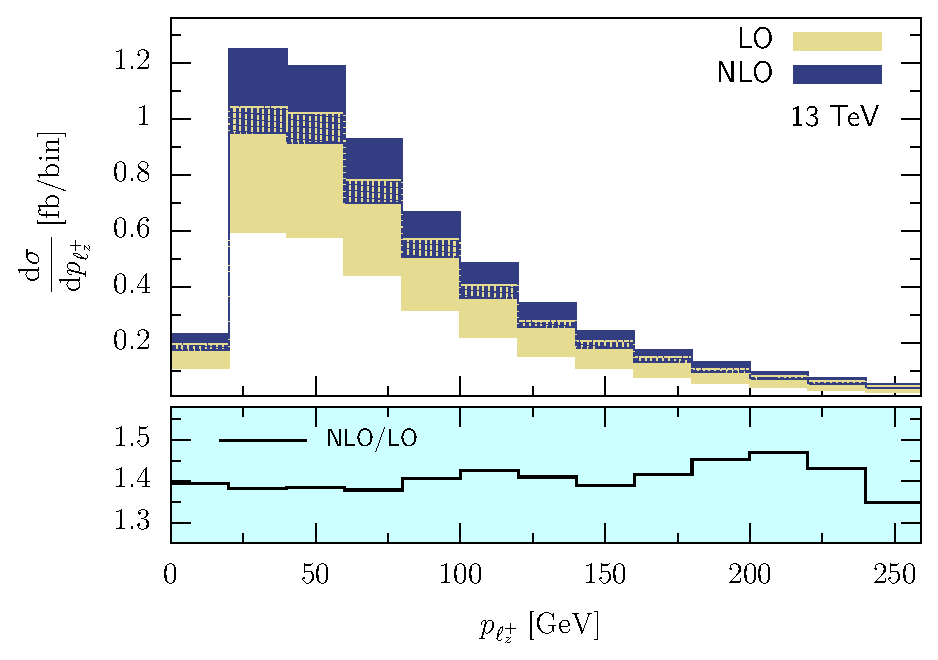
\includegraphics[width=0.45\textwidth]{./LHC_53_Fig03.eps}
\caption{\label{fig:i} Caption here.}
\end{figure}


\begin{figure}[h]
\centering % \begin{center}/\end{center} takes some additional vertical space
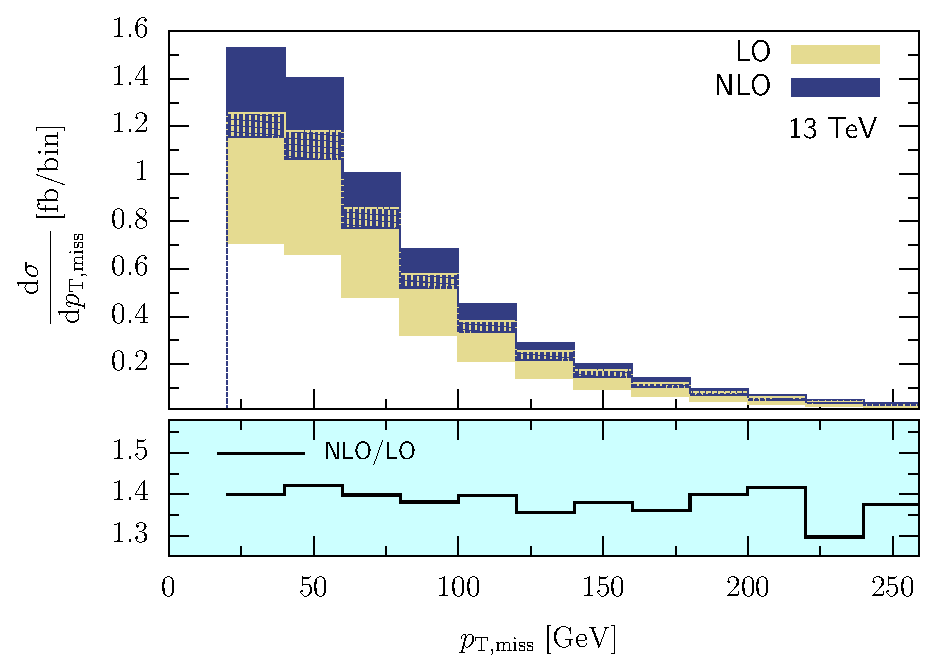
\includegraphics[width=0.45\textwidth]{./LHC_53_Fig08.eps}
\hfill
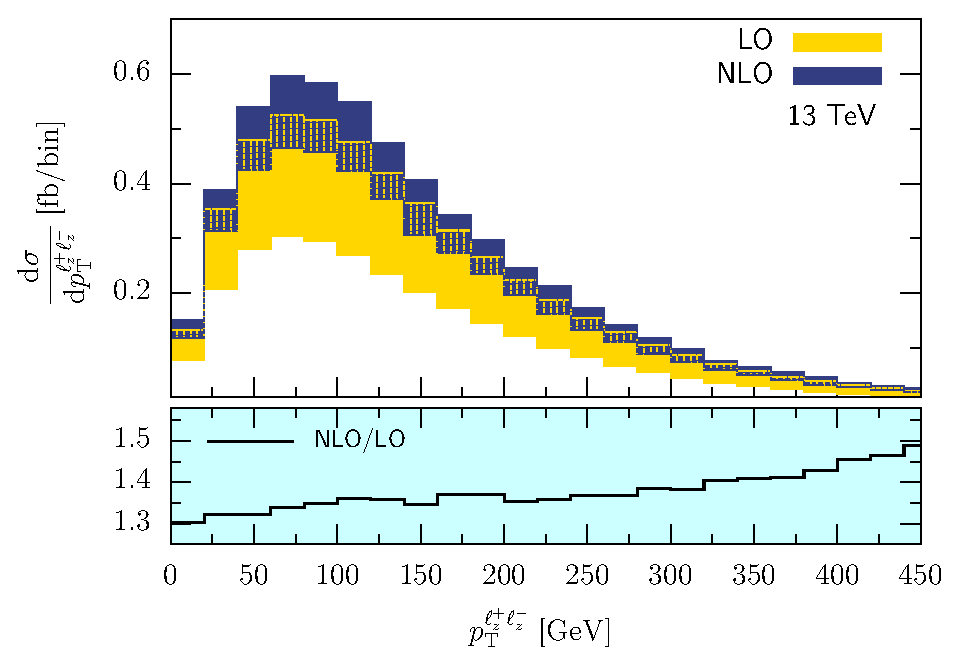
\includegraphics[width=0.45\textwidth]{./LHC_53_Fig12.eps}
\caption{\label{fig:i} Caption here.}
\end{figure}



\begin{figure}[h]
\centering % \begin{center}/\end{center} takes some additional vertical space
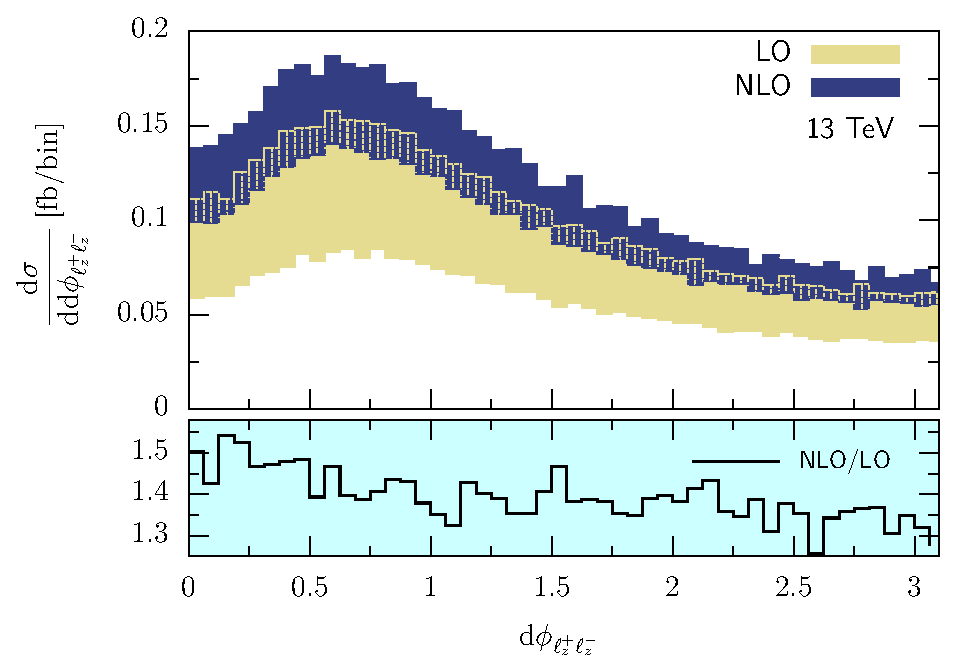
\includegraphics[width=0.45\textwidth]{./LHC_53_Fig17.eps}
\hfill
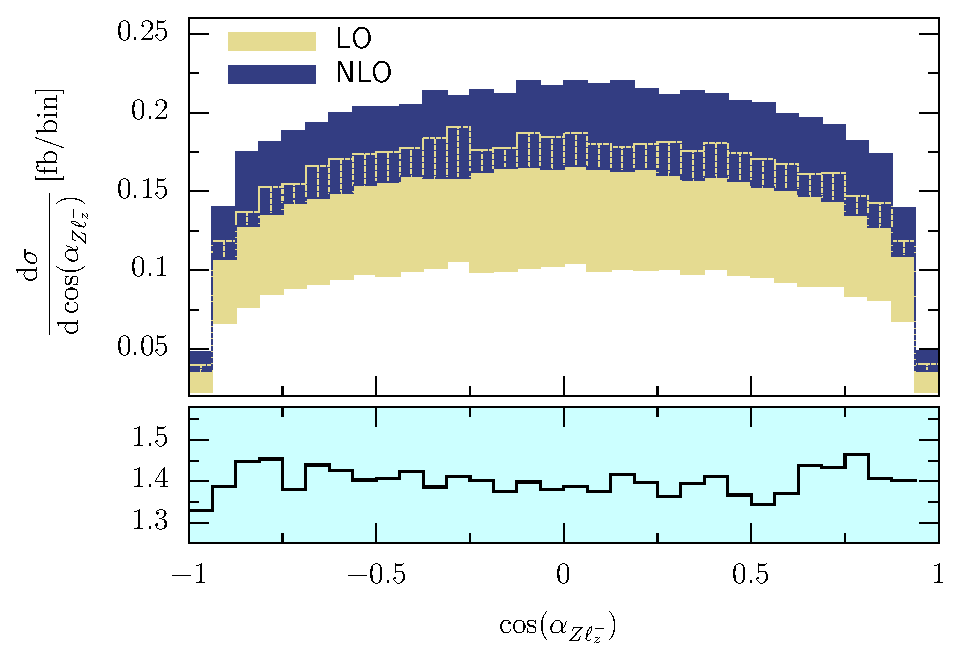
\includegraphics[width=0.45\textwidth]{./LHC_53_Fig18.eps}
\caption{\label{fig:i} Caption here.}
\end{figure}




\begin{figure}[h]
\centering % \begin{center}/\end{center} takes some additional vertical space
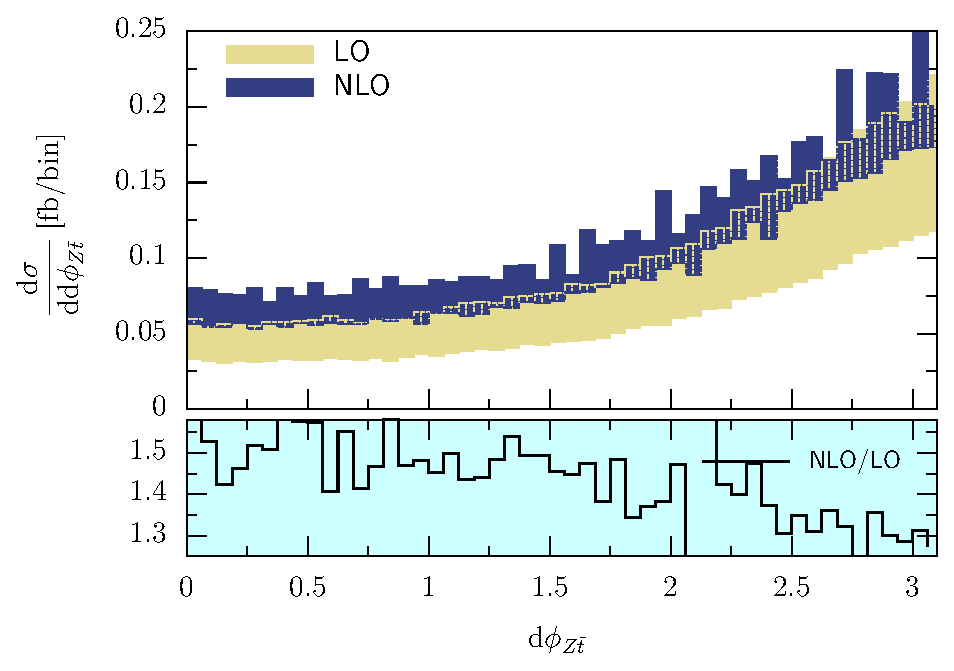
\includegraphics[width=0.45\textwidth]{./LHC_53_Fig19.eps}
\caption{\label{fig:i} Caption here.}
\end{figure}


\bibliographystyle{JHEP}
\bibliography{ttbZ}

%\begin{thebibliography}{99}

%\cite{Campbell:2013yla}
%\bibitem{Campbell:2013yla} 
%  J.~Campbell, R.~K.~Ellis and R.~Rontsch,
%  %``Single top production in association with a Z boson at the LHC,''
%  Phys.\ Rev.\ D {\bf 87}, 114006 (2013)
%  [arXiv:1302.3856 [hep-ph]].
%  %%CITATION = ARXIV:1302.3856;%%
%\end{thebibliography}

\end{document}








